\documentclass[letterpaper,10pt]{article}
\usepackage{fullpage}
\usepackage{authblk}
\usepackage{abstract}
\usepackage{appendix}
\usepackage{subcaption}
\usepackage{xspace}
\usepackage{graphicx}
\usepackage{amsmath,amssymb}
\usepackage{xcolor}
\usepackage{url}
\usepackage[htt]{hyphenat}

% algorithm stuff
\usepackage[noend]{algpseudocode}
\usepackage[ruled, vlined]{algorithm2e}
\newcommand{\myalgorithm}{
\SetKwProg{Procedure}{Procedure}{}{}
\SetKwProg{Function}{Function}{}{}
\SetKwProg{Iblock}{}{}{}
\DontPrintSemicolon
}
\newcommand\mycommfont[1]{\footnotesize\ttfamily\textcolor{blue}{#1}}
\SetCommentSty{mycommfont}


\makeatletter
\renewcommand\AB@affilsepx{, \protect\Affilfont}
\makeatother

\newtheorem{property}{Property}

\newcommand{\rust}[1]{\ensuremath{\mathtt{#1}}\xspace}
\newcommand{\module}[1]{\textcolor{orange}{\ensuremath{\mathbf{\mathsf{#1}}}\xspace}}
\newcommand{\preferred}{\rust{preferred\_round}}
\newcommand{\processcerts}{\rust{process\_certificates}}


\begin{document}
\title{State Synchronization and Verification of Committed Information in a System with Reconfigurations}
\author{}
\date{}
\maketitle

\begin{abstract}
In this document we describe the current approach for state synchronization and verification of committed transactions in case the active set of validators and their signatures can change periodically.
\end{abstract}

\section{Introduction}
\label{intro}
Below we give a brief overview of the actors and their verification operations that are relevant in light of reconfigurations in the system.

\begin{figure}[ht]
	\centering
	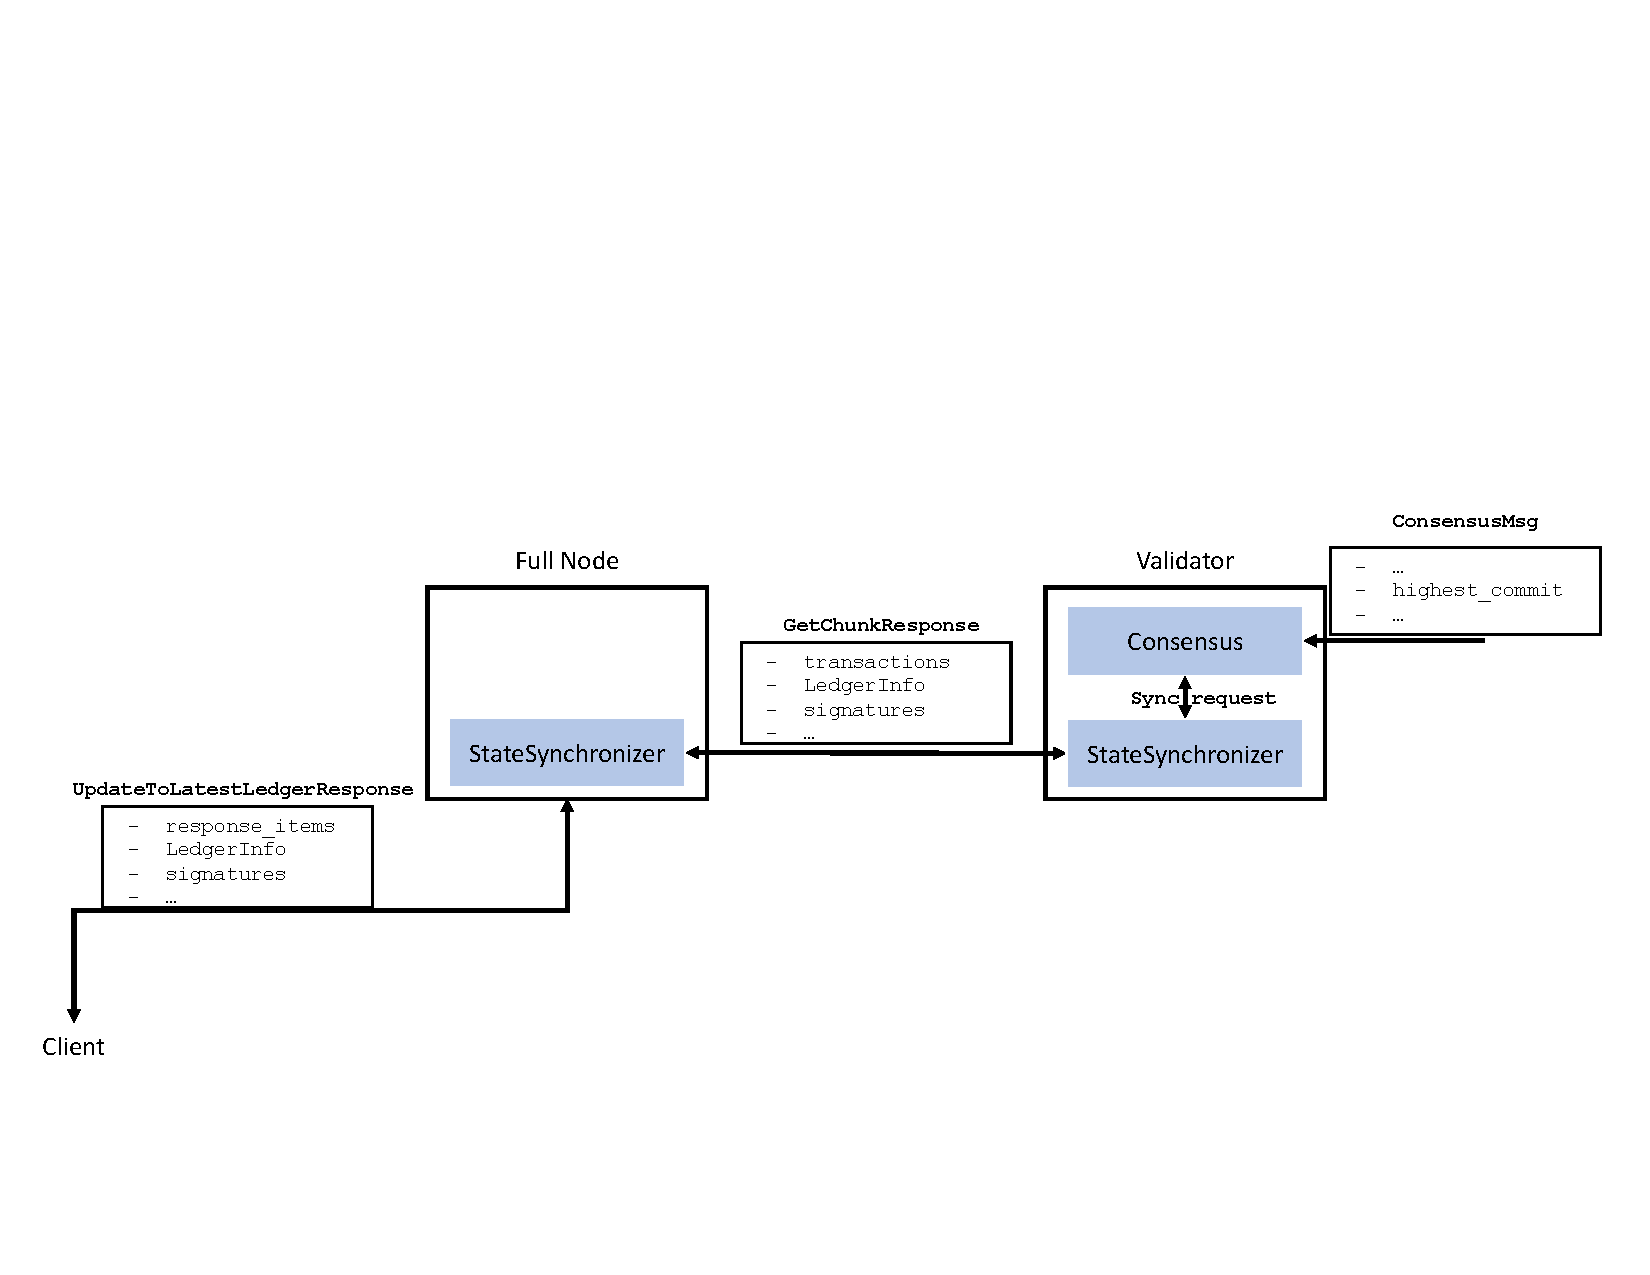
\includegraphics[width=\textwidth]{figures/verification-actors.pdf}
	\caption{\footnotesize{Main participants during verification and state sync}}
	\label{fig:verification-actors}
\end{figure}

\begin{itemize}
\item \textbf{Clients} learn about the state of the blockchain via the \texttt{UpdateToLatestLedgerRequest} and \texttt{UpdateToLatestLedgerResponse} messages. The response includes the \texttt{LedgerInfo} signed by the validator set of a given epoch (a client should have an ability to verify this validator set, see below). All the items in the response have merkle tree proofs relative to the version of the signed \texttt{LedgerInfo}.
\item \textbf{StateSynchronizer} module is used by both the validators and full nodes: it is responsible to sync up the local storage to a given remote via the \texttt{GetChunkRequest} and \texttt{GetChunkResponse} messages. The \texttt{GetChunkResponse} includes the \texttt{LedgerInfo} signed by the validator set of a given epoch and a chunk of transactions with a merkle tree range proof relative to the version of that ledger info. Upon receiving a chunk response, \texttt{StateSynchronizer} verifies the signatures of the ledger info, verifies the range tree proof, applies the transactions locally and adds the \texttt{LedgerInfo} to the local storage in case it matches the local accumulator state. There is exactly one (latest) \texttt{LedgerInfo} per epoch kept in storage.
\item \textbf{Consensus} module is run by the validators: it is using the state synchronizer to sync up the local storage in case one of the received consensus messages indicates that the peer's committed version is higher than the information stored in the local consensus speculative tree. In this case Consensus requests \texttt{StateSynchronizer} to sync up to a specific version, for which it has received a valid \texttt{LedgerInfo}.
\end{itemize}

\section{Verification through epochs}
\label{verification-epochs}

\begin{figure}[ht]
	\centering
	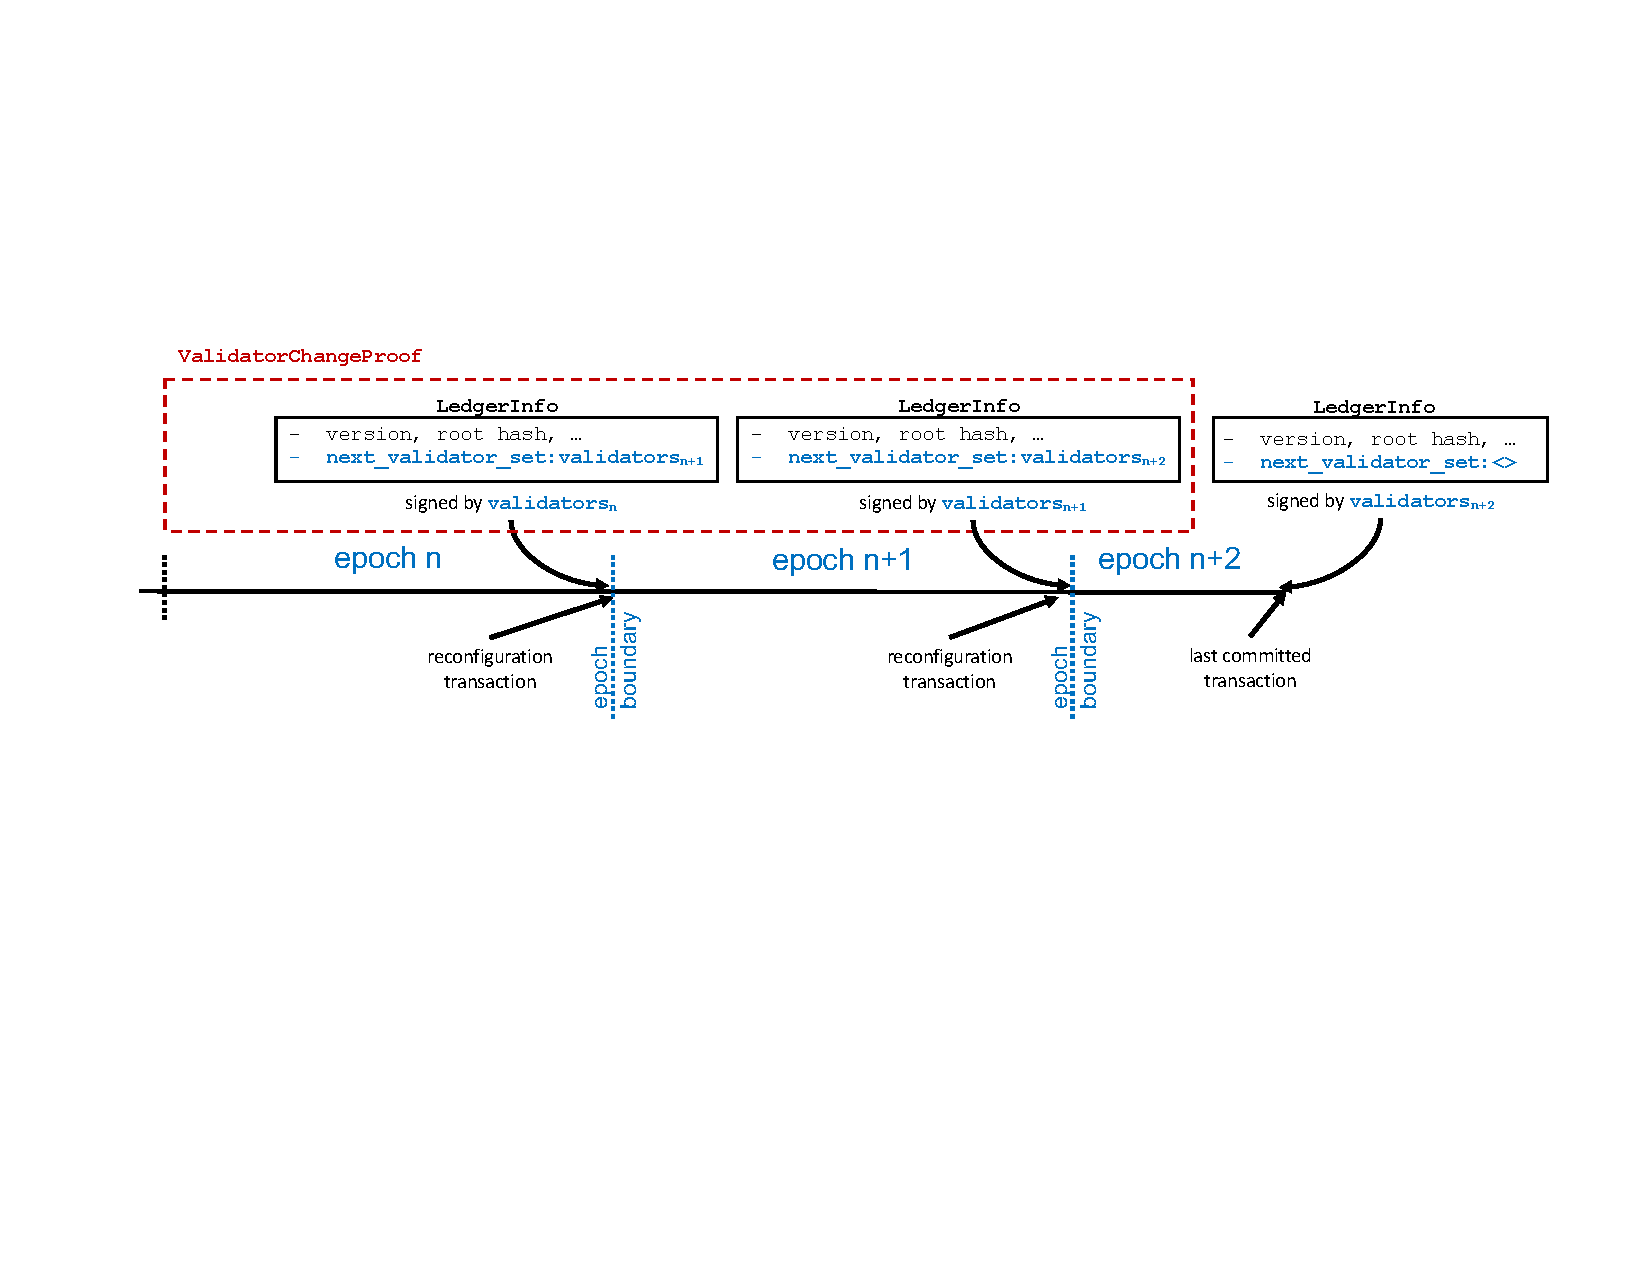
\includegraphics[width=\textwidth]{figures/ledger-store.pdf}
	\caption{\footnotesize{Latest \texttt{LedgerInfo} of an epoch keeps a validator set for the next epoch, forming a \texttt{EpochChangeProof} chain.}}
	\label{fig:ledger-store}
\end{figure}

Fundamentally, each change in the validator set is part of the state managed by the ledger. In order to simplify the protocol the new validator set is also included in the last \texttt{LedgerInfo} of each epoch in a special field \texttt{next\_validator\_set}. As shown in Figure~\ref{fig:ledger-store}, storage keeps last \texttt{LedgerInfo} for every epoch, forming a \texttt{EpochChangeProof} chain, in which each new validator set is verified using the public keys of the previous validator set.

The \texttt{EpochChangeProof} chain is included in the \texttt{UpdateToLatestLedgerResponse}, hence every participant in the system can maintain the uptodate validator set (given a trusted validator set $VS_i$ one can verify a \texttt{LedgerInfo} with a non-empty \texttt{next\_validator\_set} and thus update its trusted validator set to $VS_{i+1}$). Note that this approach assumes \textbf{some initial} trusted validator set, a challenge thoroughly described in Section~\ref{waypoints}.

\subsection{State Synchronization through epochs}
\label{state-sync-epochs}
\texttt{StateSynchronizer} could verify the latest \texttt{LedgerInfo} similarly to the way it is done by the clients described above. However, this verification might not be enough: in order for a node to be able to serve state-synchronization to its downstream peers it should store all the end-of-epoch \texttt{LedgerInfos} as well.

Thus, the sync up protocol of \texttt{StateSynchronizer} makes sure that both the transactions and the \texttt{EpochChangeProof} are properly synchronized. The downstream peer is managing the known epoch and version; the upstream peer makes sure to deliver all the end-of-epoch \texttt{LedgerInfos} (see Figure~\ref{fig:state-sync-epochs}):

\begin{figure*}[ht]
    \centering
    \begin{subfigure}{0.47\textwidth}
        \centering
        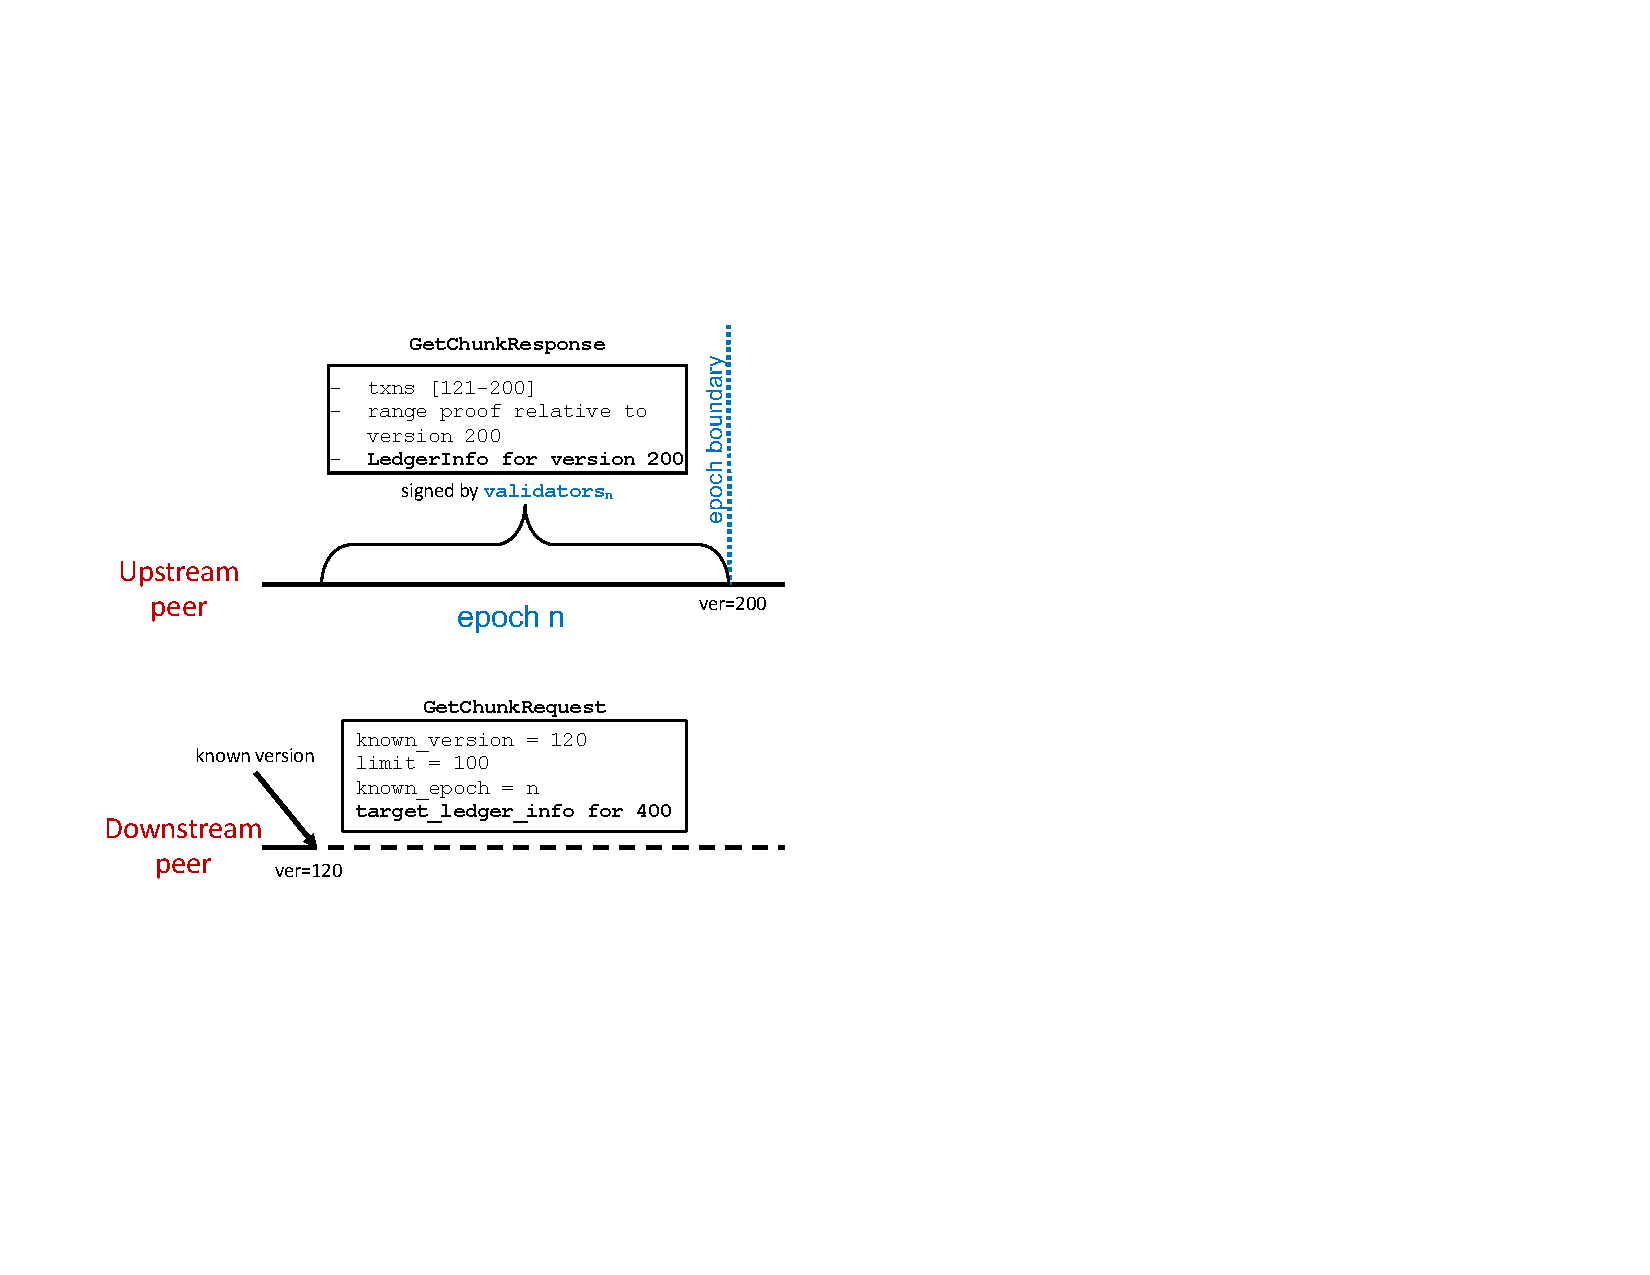
\includegraphics[height=0.8\textwidth]{figures/state-sync-epochs-1.pdf}
        \caption{\footnotesize{The \texttt{LedgerInfo} in response is determined by the last version of the request epoch.}}
        \label{fig:state-sync-epochs-1}
    \end{subfigure}
    \begin{subfigure}{0.47\textwidth}
        \centering
        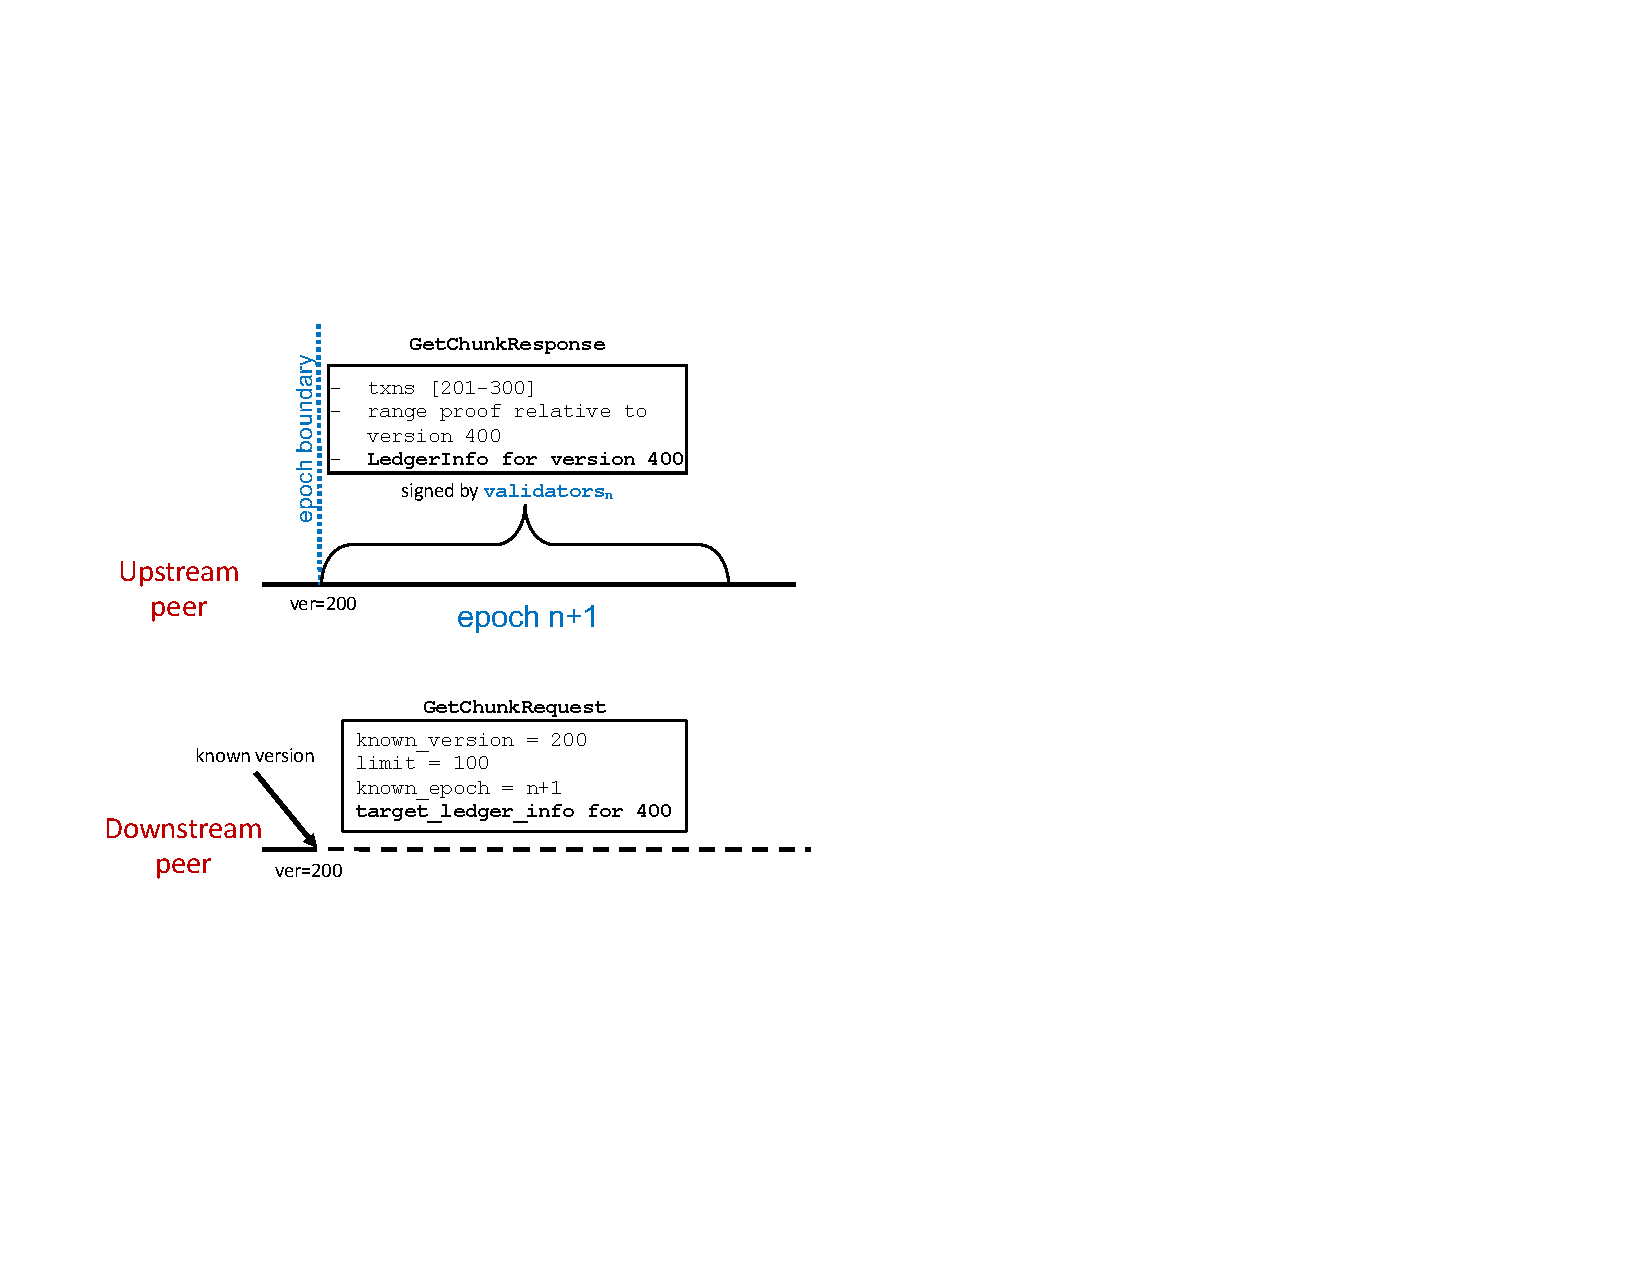
\includegraphics[height=0.8\textwidth]{figures/state-sync-epochs-2.pdf}
        \caption{\footnotesize{The \texttt{LedgerInfo} in response is determined by the target LedgerInfo of the request.}}
        \label{fig:state-sync-epochs-2}
    \end{subfigure}
    \caption{\footnotesize{Response chunks do not cross epoch boundaries and carry proofs relative to the \texttt{LedgerInfo} of the chunk's epoch.}}
    \label{fig:state-sync-epochs}
\end{figure*}

\begin{itemize}
\item \texttt{GetChunkRequest} carries the information about the known version and epoch of the requester.
\item \texttt{GetChunkResponse} carries chunks that never cross epoch boundaries. In case a chunk terminates the epoch it belongs to, the \texttt{LedgerInfo} in the chunk also includes the \texttt{next\_validator\_set}, which helps the receiver to move to the next epoch (Figure~\ref{fig:state-sync-epochs-1}).
\item One interesting aspect worth noting here is that in case a state synchronization request has a predefined target, the chunk response carries either the \texttt{LedgerInfo} of the given target, or the last \texttt{LedgerInfo} of the request epoch (the smaller between the two), to make sure that the receiver can still verify the response as depicted in Figure~\ref{fig:state-sync-epochs}. In these cases the chunk can be smaller than the max allowed chunk size, just to make sure that the chunks do not cross epoch boundaries.
\item The receiver of the \texttt{GetChunkResponse} executes the following verification steps:
\begin{itemize}
\item Verify the signatures of the response \texttt{LedgerInfo} using the current validator set (chunk response must belong to the epoch of the request).
\item Verify the merkle range proof of the chunk transactions relative to the \texttt{LedgerInfo} of the response.
\item Apply the transactions to the local accumulator.
\item Verify that the local accumulator state matches the metadata of the response \texttt{LedgerInfo} and add this \texttt{LedgerInfo} to the local storage.
\end{itemize}
\end{itemize}

\section{Waypoints}
\label{waypoints}
\subsection{Motivation}
\label{waypoint-motivation}
A \emph{cold} node (the one that comes online for the first time, or after a long period of being disconnected), faces a problem of the initial syncup because it might no longer trust the old public keys of the historical validators it is aware of, which could have been compromised since then (the so called “long range attack”).

\emph{Waypoints} can be used  as an off-chain mechanism for selecting the initial trusted set of validators and specific points in the accumulator history. Waypoints can be published by anyone. The Libra Association is also expected to publish waypoints on a regular basis (e.g., on \url{https://developers.libra.org}). Any waypoint selected by clients can be embedded within the nodes (clients / full nodes / validators) as a trusted “starting point”.

The trusted points in history determined by the waypoints can be used in the following situations:
\begin{itemize}
\item \textbf{Long range attacks}: trusted recovery relative to a recent point in time for a cold node that does not have an up-to-date information locally.
\item \textbf{Genesis configuration}: a genesis waypoint certifies the genesis \texttt{LedgerInfo} with its initial validator set.
\item \textbf{Emergency reconfigurations}: consider a disastrous scenario, in which a reconfiguration must be applied without an ability to generate a \texttt{LedgerInfo} with a valid set of signatures (e.g., private keys are lost, or the system needs to be forcefully upgraded to a previous point in time). The \texttt{LedgerInfo} of this reconfiguration cannot be verified via the standard signature checks, and it's going to be verified using waypoints (see more in Section~\ref{waypoint-emergency}).
\end{itemize}

Obviously, being an off-chain mechanism there is no way to “prove” a waypoint, the nodes choose to trust waypoints for their initialization.

\subsection{Waypoint structure}
\label{waypoint-structure}
In order to provide a client with the initial trusted root hash and validators, it is enough for the waypoint to include the information about a LedgerInfo on the epoch boundary (the one that must include the validator set of the next epoch).

The waypoint representation remains a short string that can be easily included in a config or copied from an association website.

\begin{algorithm}[H]
\myalgorithm
{
\Iblock{\rust{Waypoint}}{
	   \tcp{The version of the reconfiguration transaction that is being approved by this waypoint.}
        \rust{version: u64}\;
        \tcp{The hash of the chosen fields of LedgerInfo (including the next epoch info).}
        \rust{value: HashValue}
}
}
\end{algorithm}


The fields of a LedgerInfo that are included in the waypoint value are \texttt{epoch}, \texttt{root\_hash}, \texttt{version}, \texttt{timestamp}, and \texttt{next\_validator\_set}. Note that we cannot include all the fields because they might not be deterministic: different clients might observe different values of e.g., \texttt{consensus\_block\_id} of the latest \texttt{LedgerInfo} in an epoch.

The textual representation of a Waypoint is  "version:hex encoding of the root hash". For example, the current testnet genesis waypoint is \newline \texttt{"0:a17035961b97359bcc22b628c1e269f543b265220d22a17e4a5b4e3aed86855b"}.

\subsection{Verifying the latest LedgerInfo with waypoints}
\label{waypoint-li-verification}
As described in Section~\ref{verification-epochs}, an \texttt{UpdateToLatestLedgerResponse} message carries a data structure for verifying validator changes, \texttt{EpochChangeProof}, which contains a list of all the epoch change \texttt{LedgerInfos}. A client verifies this list in an iterative fashion starting with its initial trusted \texttt{ValidatorSet}.

\begin{figure}[ht]
	\centering
	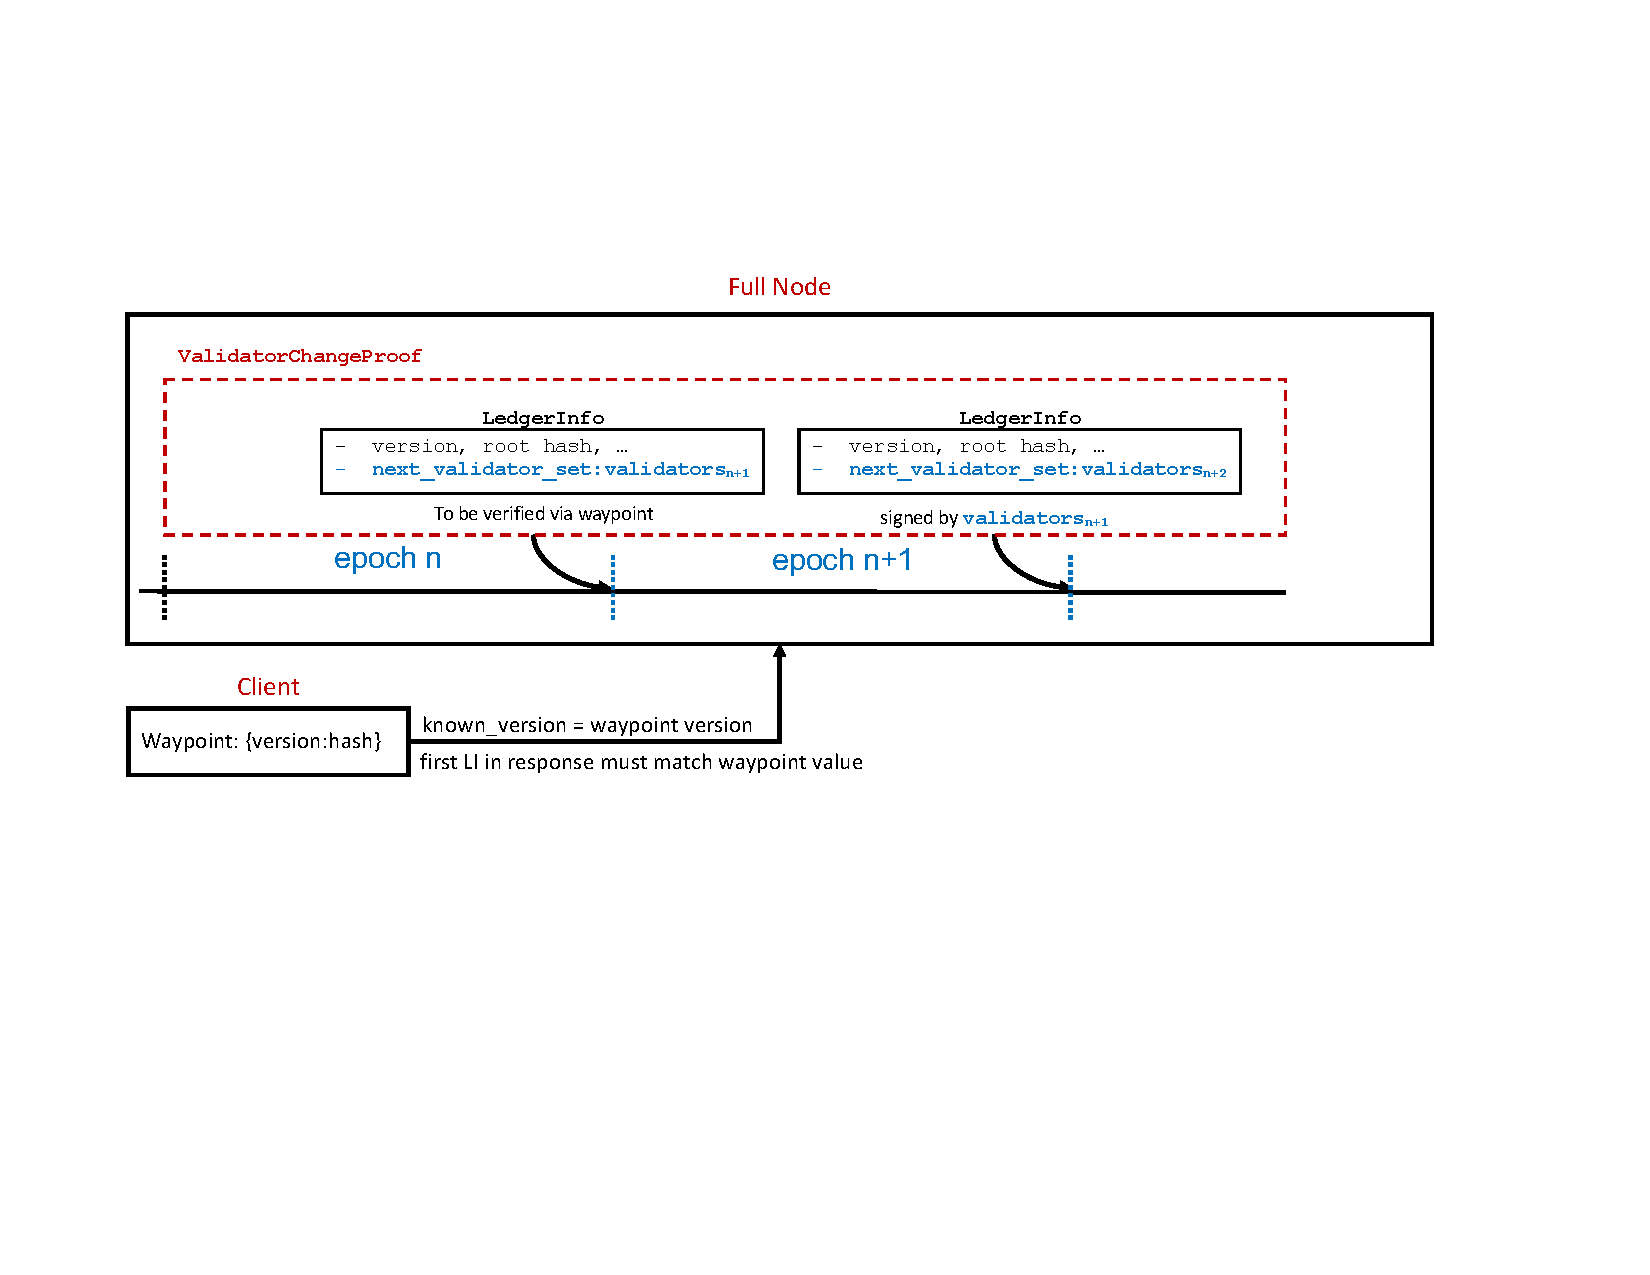
\includegraphics[width=\textwidth]{figures/waypoint-verification.pdf}
	\caption{\footnotesize{The first LedgerInfo in the \texttt{EpochChangeProof} is verified via a local waypoint.}}
	\label{fig:waypoint-verification}
\end{figure}

Waypoint verification is working slightly differently as shown in Figure~\ref{fig:waypoint-verification}.
A waypoint version corresponds to the last version of an epoch (version $0$ being somewhat special and corresponding to the last and only version of epoch $0$).
Hence, the \texttt{EpochChangeProof} in the response starts with the end-of-epoch \texttt{LedgerInfo} corresponding to the waypoint: this very first \texttt{LedgerInfo} is verified using the waypoint. The rest of the epoch changes is verified in a regular manner.

\subsection{State synchronization with waypoints}
\label{waypoint-state-sync}
As described in Section~\ref{state-sync-epochs}, a node should possess the intermediate end-of-epoch \texttt{LedgerInfos} in order to be able to serve its downstream peers.
Consider a following scenario:
\begin{itemize}
\item Full node $A$ has reached epoch $100$.
\item Full node $B$ is a downstream peer of $A$ that is restarted with waypoint $W_{80}$ corresponding to the last version of epoch $80$.
\item Full node $C$ is a downstream peer of $B$ that is restarted with waypoint $W_{60}$ corresponding to the last version of epoch $60$.
\end{itemize}

Waypoints are not transferable: the fact that $B$ has decided to trust a waypoint $W_{80}$ does not mean it can send this waypoint to $C$, which might still trust $W_{60}$ only. Hence, $B$ needs to be able to prove validator changes to $C$ in the epoch range $60-80$, therefore it must bring the intermediate end-of-epoch \texttt{LedgerInfos} in a verifiable manner.

Unlike the protocol described in Section~\ref{state-sync-epochs}, the verification of intermediate end-of-epoch \texttt{LedgerInfos} \textbf{prior} to the waypoint (epochs below $80$ in our example) cannot be based on signature verification, because $B$ does not trust the old signatures. The verification of pre-waypoint items is relative to this waypoint:

\begin{figure}[ht]
	\centering
	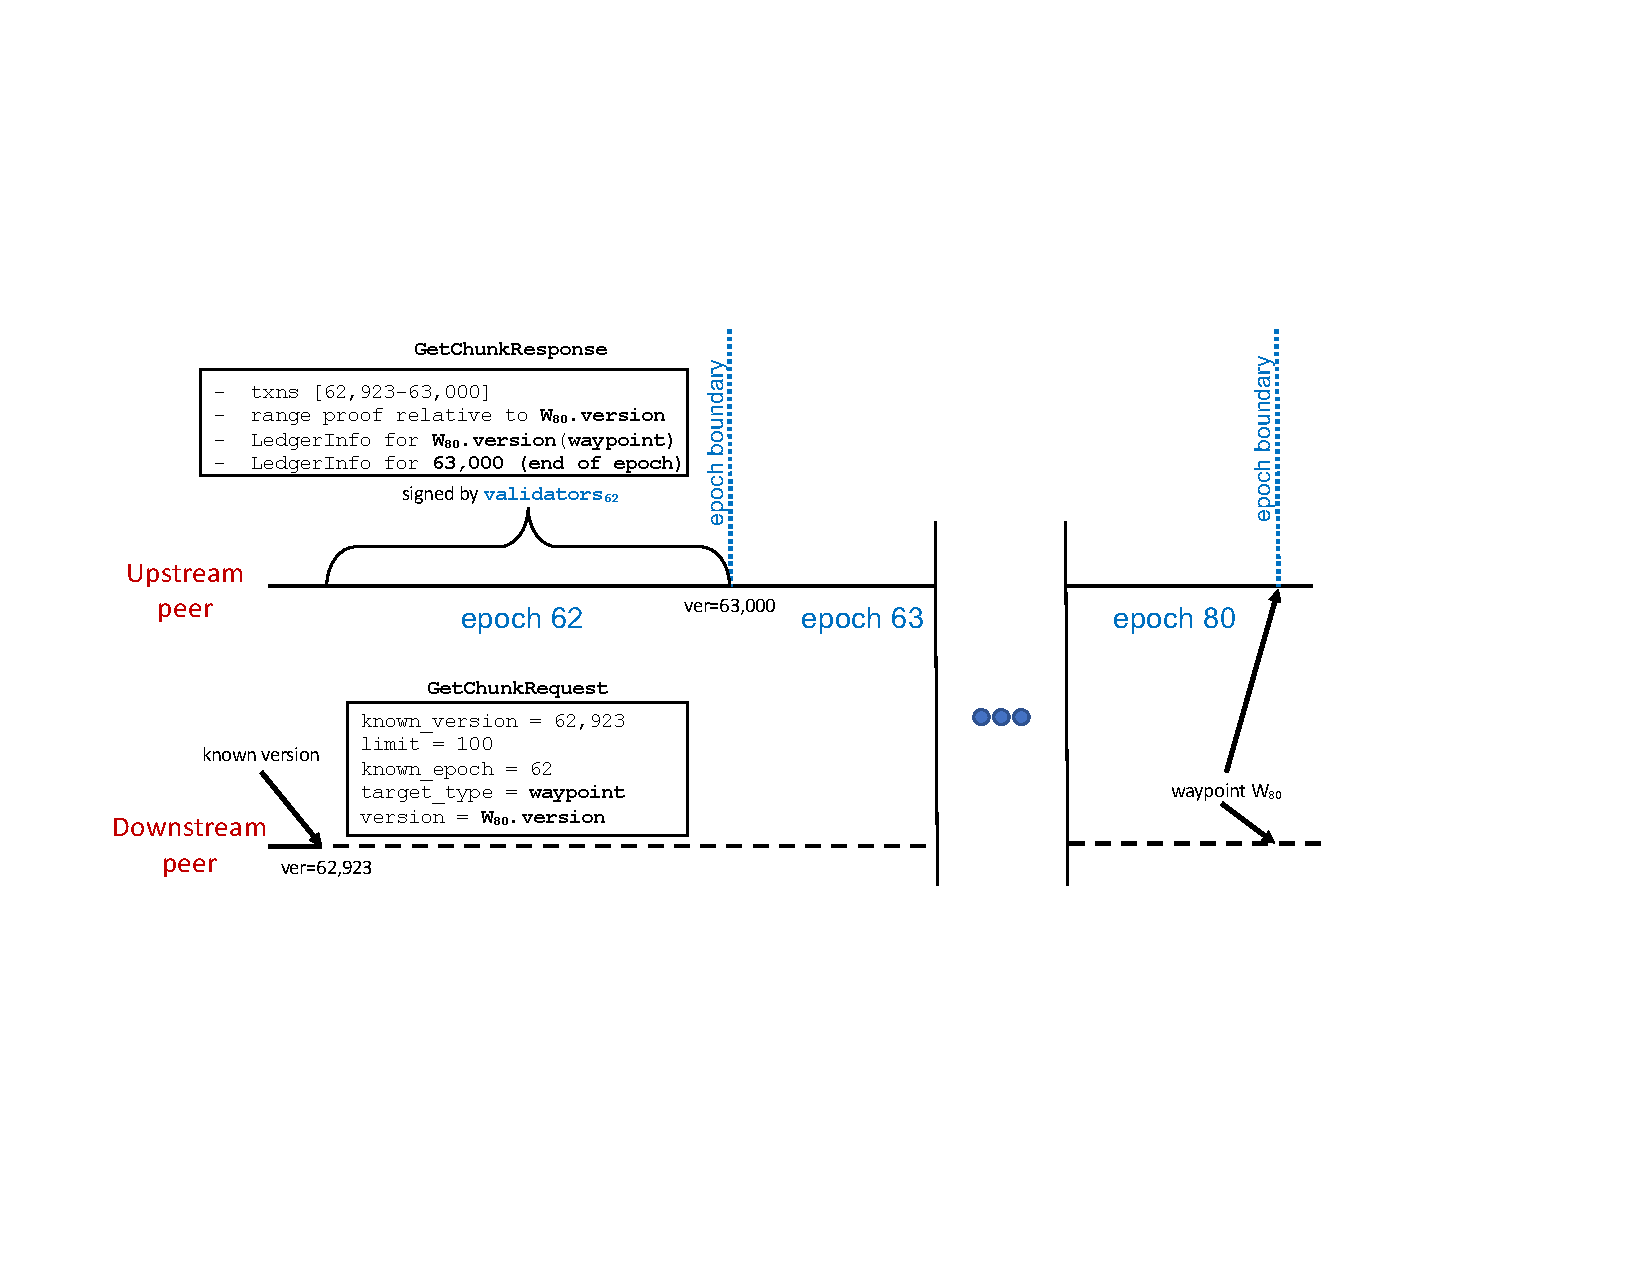
\includegraphics[width=\textwidth]{figures/state-sync-waypoint.pdf}
	\caption{\footnotesize{ChunkResponse carries the LI of a waypoint and an optional intermediate end-of-epoch LI.}}
	\label{fig:state-sync-waypoint}
\end{figure}

\begin{itemize}
\item \texttt{GetChunkRequest} specifies the target type to be a \texttt{waypoint} with the version corresponding ot the version of the local waypoint.
\item Each chunk response carries a \texttt{LedgerInfo} determined by the target waypoint version. This \texttt{LedgerInfo} is verified using a waypoint.
\item The range of transactions in the response chunk carries a merkle tree proof relative to the version of the waypoint as well.
\item The chunks that are sent back never cross epoch boundaries.
\item In case the chunk terminates an intermediate epoch (e.g., a last chunk of epoch $62$ in Figure~\ref{fig:state-sync-waypoint}), the chunk response carries an intermediate end-of-epoch \texttt{LedgerInfo}.
\item The receiver of such a chunk first executes the transactions and then verifies that the root hash and the metadata of the intermediate end-of-epoch \texttt{LedgerInfo} indeed correspond to its local accumulator state. In such case this end-of-epoch \texttt{LedgerInfo} is added to the local ledger store and can later be used for providing state synchronization to the downstream nodes.
\end{itemize}

\subsection{Consensus and TCB initialization with waypoints}
\label{waypoint-tcb}
In this section we briefly describe the way consensus and TCB components utilize the waypoint mechanism during startup.

Consensus component trusts its local State Synchronizer. The startup order makes sure that Consensus starts only after State Synchronizer is fully initialized. In case a validator starts with a waypoint that is higher than the latest version stored in its local storage, the following chain of events occurs:
\begin{itemize}
\item State Synchronizer retrieves all the committed information up to the waypoint, as described in Section~\ref{waypoint-state-sync}, and then considers itself initialized.
\item Consensus starts after the initialization of State Synchronizer is complete and looks for the new root.
\item Consensus detects that 1) the highest \texttt{LedgerInfo} in its local storage is higher than the previously stored consensus root, and 2) this \texttt{LedgerInfo} keeps the validator set for the next epoch (waypoint is set at the epoch change boundary). In this case, Consensus generates a new genesis block and starts a new epoch.
\end{itemize}

Unlike Consensus, TCB does not trust any other component in the system, hence, it keeps the waypoint of its own (in its local TCB config). Upon startup TCB verifies the latest \texttt{LedgerInfo} in the local store using its own waypoint (one should be careful to maintain the TCB and State Synchronizer waypoint copies identical because otherwise the startup verification might fail). TCB does not need to verify all the previous end-of-epoch \texttt{LedgerInfos} prior to its waypoint because it is not responsible for the synchronization services.

\begingroup
\bibliographystyle{plain}
\bibliography{citations}
\endgroup

\end{document}
